\documentclass[../main.tex]{subfiles}
\begin{document}

In der Bewertung der Ergebnisse muss nun auf Grundlage der erzeugten Datei die Entscheidung getroffen, ob der Code compliant oder nicht ist.
Bisher wurde diese Entscheidung nicht nach klaren Richtlinien getroffen.
Stattdessen wurde sie von dem Piper übernommen.
Problem ist, dass dieser Prozess mit Piper nicht durchsichtig ist und keine Verantwortungen eindeutig geklärt sind.
Es bedarf einer Lösung, die flexibel, falls sich die Anforderungen an Code und damit die Richtlinien ändern, und nachvollziehbar, sodass immer klar ist auf welcher Grundlage die Entscheidung getroffen wurde, ist.

Von der SAP Abteilung Hyperspace werden seit neusten Richtlinien in einem \gls{glos:PolicyAsCode} Format bereitgestellt.
Diese Richtlinien sind in der sogenannten Rego Programmiersprache formuliert, die mit dem \gls{OPA} angewandt werden können.
Dieser \gls{OPA} wird wiederum von Hyperspace genutzt.

\begin{figure}[ht]
    \centering
    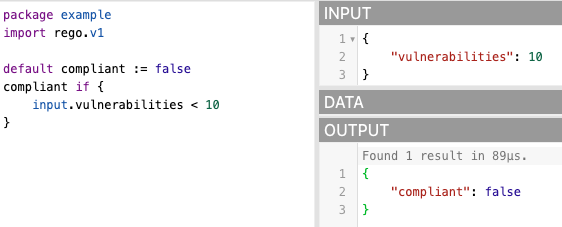
\includegraphics[scale=0.65]{bilder/regoexample.png}
    \caption{Beispiel Rego Script mit Ein- und Ausgabe (selbst geschrieben)}
    \label{fig:regoexample}
\end{figure}

Das in Abbildung \ref{fig:regoexample} zu sehende Script ist immer eindeutig, transparent und schnell anzupassen.
Die verwendete Rego Programmiersprache ist außerdem dafür optimiert Richtlinien anzuwenden.
Damit is der \gls{OPA} mit Rego für die genannten Anforderungen geeignet.
\cite{Rego}

\end{document}